\documentclass[a4paper]{article}
\usepackage[T1]{fontenc}			% pacchetto per \chapter
\usepackage[italian]{babel}
\usepackage[italian]{isodate}  		% formato delle date in italiano
\usepackage{graphicx}				% gestione delle immagini
\usepackage{amsfonts}
\usepackage{booktabs}				% tabelle di qualità superiore
\usepackage{amsmath}				% pacchetto matematica
\usepackage{mathtools}				% per sottolineare sotto le equazioni
\usepackage{stmaryrd} 				% per '\llbracket' e '\rrbracket'
\usepackage{amsthm}					% teoremi migliorati
\usepackage{enumitem}				% gestione delle liste
\usepackage{pifont}					% pacchetto con elenchi carini
\usepackage{enumitem}				% pacchetto per elenchi con lettere dell'alfabeto
\usepackage{cancel}					% per cancellare delle espressioni matematiche
\usepackage{listings}				% implementa codice di programmazione


\usepackage[x11names]{xcolor}		% pacchetto colori RGB
% Link ipertestuali per l'indice
\usepackage{xcolor}
\usepackage[linkcolor=black, citecolor=blue, urlcolor=cyan]{hyperref}
\hypersetup{
	colorlinks=true
}

% Colour code style
\definecolor{codegreen}{rgb}{0,0.6,0}
\definecolor{codegray}{rgb}{0.5,0.5,0.5}
\definecolor{codepurple}{rgb}{0.58,0,0.82}
\definecolor{backcolour}{rgb}{0.95,0.95,0.92}

\lstdefinestyle{MATLAB}{
	backgroundcolor=\color{backcolour},   
	commentstyle=\color{codegreen},
	keywordstyle=\color{magenta},
	numberstyle=\tiny\color{codegray},
	stringstyle=\color{codepurple},
	basicstyle=\ttfamily\footnotesize,
	breakatwhitespace=false,         
	breaklines=true,                 
	captionpos=b,                    
	keepspaces=true,                 
	numbers=left,                    
	numbersep=5pt,
	showspaces=false,                
	showstringspaces=false,
	showtabs=false,                  
	tabsize=2
}
\lstset{style=MATLAB}

%\usepackage{showframe}				% visualizzazione bordi
%\usepackage{showkeys}				% visualizzazione etichetta

\newtheorem{theorem}{\textcolor{Red3}{\underline{Teorema}}}
\newtheorem{lemma}{Lemma}
\renewcommand{\qedsymbol}{QED}
\newcommand{\exec}[1]{\llbracket #1\:\rrbracket}
\newcommand{\dquotes}[1]{``#1''}
\newcommand{\longline}{\noindent\rule{\textwidth}{0.4pt}}

\begin{document}
	\author{Università degli Studi di Verona}
	\title{Simulazione di Elaborazione di segnali e immagini}
	\date{{\Large 26 Marzo 2021}}
	\maketitle
	
	\section{Esercizio}
	
	Siano $x\left(t\right)$ un segnale di durata indefinita il cui spettro analitico $X\left(\mu\right)$ è rappresentato in figura 1.
	\begin{figure}[!htp]
		\centering
		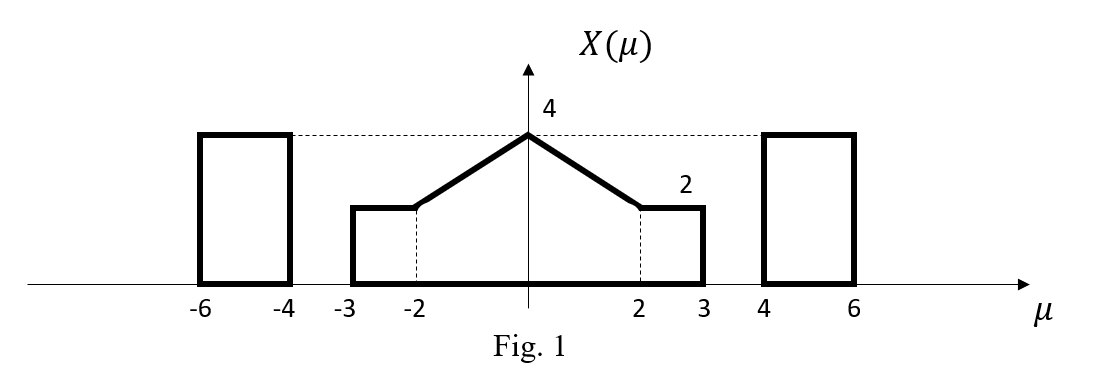
\includegraphics[width=\textwidth]{img/fig_1.png}
	\end{figure}

	\begin{itemize}
		\item Descrivere analiticamente, nel \underline{tempo} ed in \underline{frequenza} il segnale $X\left(\mu\right)$;
		
		\item Descrivere analiticamente e graficamente, in \underline{frequenza}, i segnali $a\left(t\right), b\left(t\right), c\left(t\right), d\left(t\right)$ ottenuti come descritto nel sistema in figura 2, considerando [fc] come la frequenza di campionamento minima per la quale il segnale $b\left(t\right)$ è replicato senza ottenere alcun effetto di aliasing, facendo le assunzioni necessarie sugli estremi del segnale.
	\end{itemize}
	\begin{figure}[!htp]
		\centering
		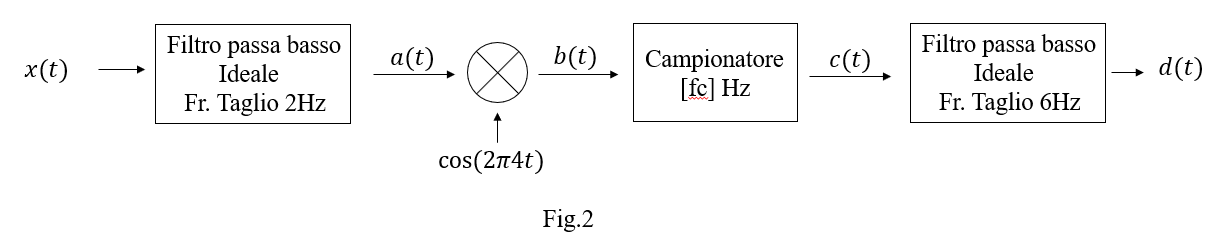
\includegraphics[width=\textwidth]{img/fig_2.png}
	\end{figure}\newpage

	\section{Esercizio}
	
	Siano $x\left(t\right)$ e $h\left(t\right)$ i due segnali nel dominio discreto del tempo raffigurati in figura 3, dove gli impulsi sono 
	segnali aventi altezza 1.
	\begin{figure}[!htp]
		\centering
		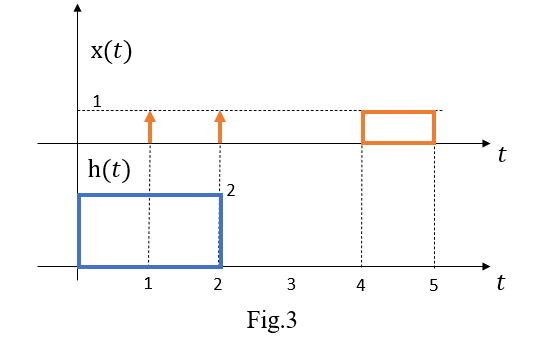
\includegraphics[width=.6\textwidth]{img/fig_3.png}
	\end{figure}
	
	\begin{itemize}
		\item Si descriva analiticamente e graficamente il segnale $y\left(t\right)$ ottenuto eseguendo la convoluzione $y\left(t\right) = x\left(t\right) * h\left(t\right)$, assumendo $h\left(0\right) = 0$
		
		\item Si raffiguri il segnale $w\left(t\right) = \Pi\left(\frac{t-4}{6}\right) - y\left(t\right)$
	\end{itemize}
	Facendo attenzione in entrambe i casi ad indicare attentamente tempo di inizio e fine del segnale, e il suo sviluppo nelle ordinate.\newpage
	
	\section{Esercizio}
	
	\begin{figure}[!htp]
		\centering
		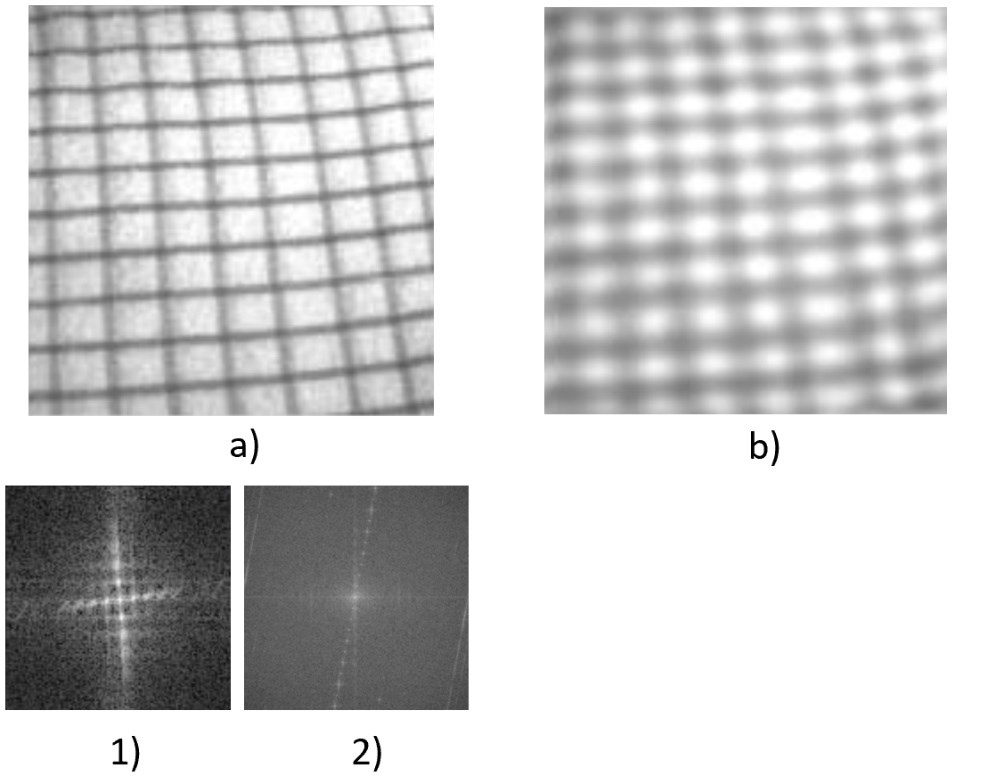
\includegraphics[width=\textwidth]{img/fig_4.png}
	\end{figure}

	\begin{enumerate}[label=\Roman*]
		\item Quali dei due spettri in ampiezza tra 1) e 2) corrispondono all'immagine a)? Perché?
		
		\item Che operazioni devo eseguire sulla rappresentazione in frequenza dell'immagine in a) per arrivare all'immagine in b)? Devo eseguire qualche operazione sullo spettro di fase dell'immagine in a) (non visualizzato in figura) per passare a b)? Perché?
	\end{enumerate}
\end{document}